\documentclass[11pt,a4paper]{article}

% --- Essential Packages ---
\usepackage[utf8]{inputenc}
\usepackage[margin=0.8in]{geometry}
\usepackage{amsmath,amssymb}
\usepackage{booktabs}
\usepackage{tabularx}
\usepackage{graphicx}
\usepackage{subcaption}
\usepackage{xcolor}
\usepackage{hyperref}
\usepackage{listings}
\usepackage{fancyhdr}
\usepackage{titlesec}
\usepackage{tikz}
\usetikzlibrary{shapes.geometric, arrows.meta, positioning, fit, backgrounds}

% --- Typography & Colors ---
\definecolor{primary}{RGB}{20, 45, 85}
\definecolor{secondary}{RGB}{35, 100, 170}
\definecolor{darkgray}{RGB}{50, 50, 50}
\definecolor{lightgray}{RGB}{245, 247, 250}
\definecolor{codebg}{RGB}{240, 242, 245}

\hypersetup{
    colorlinks=true,
    linkcolor=secondary,
    citecolor=secondary,
    urlcolor=secondary
}

% --- Code Listing Settings ---
\lstset{
    backgroundcolor=\color{codebg},
    basicstyle=\ttfamily\footnotesize,
    breaklines=true,
    captionpos=b,
    frame=single,
    rulecolor=\color{lightgray},
    numbers=left,
    numberstyle=\tiny\color{gray},
    keywordstyle=\color{primary}\bfseries,
    commentstyle=\color{gray}\itshape,
    stringstyle=\color{secondary},
    showstringspaces=false
}

% --- Header & Footer ---
\pagestyle{fancy}
\fancyhf{}
\lhead{\footnotesize Enterprise Software Development — Fall 2026}
\rhead{\footnotesize Assignment 2: HTTP, gRPC, and Metrics}
\cfoot{\thepage}

% --- Section Styling ---
\titleformat{\section}{\large\bfseries\color{primary}}{\thesection}{1em}{}
\titleformat{\subsection}{\normalsize\bfseries\color{secondary}}{\thesubsection}{1em}{}

% --- Metadata ---
\title{\vspace{-1.5cm}\textbf{\Large Enterprise Software Development (Fall 2026)}\\[0.3em]
\textbf{\LARGE Assignment 2: HTTP APIs, gRPC Services, and Metrics Observability}}
\author{\textbf{Muhammad Abdullah Khan} \\ Department of Computer Science}
\date{\today}

\begin{document}

\maketitle

\begin{abstract}
This report details the architectural enhancements made to the Bookstore Observability platform developed in Assignment 1. In Part A, we evaluate the HTTP API against REST architectural constraints, implement an OpenAPI 3.1 specification, enforce idempotent mutations, apply sliding-window rate limiting, and validate downstream resiliency using a custom Python caller implementing timeouts, exponential backoff, and a three-state circuit breaker. In Part B, we introduce a dedicated gRPC microservice sharing the identical SQLite persistence layer (configured with Write-Ahead Logging) and business rules, analyzing the semantic parity between HTTP/1.1 and HTTP/2 framing alongside status code mappings. In Part C, we audit the metric pipeline, exposing a dedicated Prometheus scrape endpoint for gRPC telemetry and designing Grafana dashboard panels that monitor RPC method rates, p50/p95 latency histograms, and active in-flight concurrency beside existing HTTP metrics.
\end{abstract}

\vspace{-0.5em}
\hrule
\vspace{1em}

% =========================================================================
% SECTION 1: PART A
% =========================================================================
\section{Part A: Improving the HTTP API}

\subsection{REST Constraints and Architectural Compliance}
Fielding's Representational State Transfer (REST) architectural style relies on six core constraints. Table~\ref{tab:rest_constraints} breaks down each constraint into plain-language terms and explains how our Bookstore API implements it, or why it was deliberately omitted.

\begin{table}[h!]
\centering
\small
\renewcommand{\arraystretch}{1.25}
\begin{tabularx}{\textwidth}{p{3.2cm} p{5.5cm} X}
\toprule
\textbf{Constraint} & \textbf{Plain-Language Meaning} & \textbf{Bookstore API Implementation} \\
\midrule
\textbf{Client-Server} & Decouples consumer interfaces from backend data storage. Either side can evolve independently without breaking contracts. & The Python callers (\texttt{caller\_http.py}, traffic generator) interact exclusively via HTTP/1.1 JSON without internal knowledge of SQLite storage. \\
\textbf{Statelessness} & Every request must contain all context required for processing. The server holds no client session state between calls. & Every request to \texttt{/books} carries its full payload, correlation ID (\texttt{x-request-id}), and \texttt{Idempotency-Key}. No session cookies or conversational server state exist. \\
\textbf{Cacheability} & Responses must explicitly mark whether they can be reused by clients or intermediate proxies to eliminate redundant roundtrips. & \texttt{GET /books} emits \texttt{Cache-Control: public, max-age=10}. Single book lookup \texttt{GET /books/\{id\}} returns \texttt{Cache-Control: public, max-age=30} with an entity tag (\texttt{ETag}). \\
\textbf{Uniform Interface} & A consistent interface contract across all endpoints via resource URIs, standard representations, self-descriptive messages, and hypermedia. & Resources use standard plural paths (\texttt{/books}). Creation returns status \texttt{201 Created} with a \texttt{Location: /books/\{id\}} header; errors strictly follow the RFC~7807 Problem Details specification. \\
\textbf{Layered System} & Intermediary components (load balancers, gateways, proxies) can be placed between client and server without the client's knowledge. & The client interacts across Docker bridge networks and middleware layers (logging, rate-limiter, error traps) without coupling to the raw database layer. \\
\textbf{Code on Demand} \newline \textit{(Optional)} & Servers temporarily extend client capabilities by transmitting executable code (e.g., scripts or applets). & \textbf{Not Demonstrated.} Marked as optional in REST principles. Our bookstore backend serves structured JSON payloads exclusively, with no script execution on the client. \\
\bottomrule
\end{tabularx}
\caption{The six REST constraints applied to the Bookstore API.}
\label{tab:rest_constraints}
\end{table}

\subsection{OpenAPI Specification (OAS 3.1) and Endpoint Verification}
The OpenAPI Specification establishes a programming-language-agnostic interface description for HTTP APIs. It allows developers and automated toolchains to discover endpoints, inspect input/output schemas, generate SDKs, and execute interactive tests without access to source code.

Our API defines declarative Pydantic schemas and metadata annotations in \texttt{app.py}, exporting an OpenAPI 3.1 specification at \texttt{/openapi.json}. The interactive Swagger UI is exposed at \texttt{/docs}. Figure~\ref{fig:swagger_overview} illustrates the generated Swagger UI interface.

\begin{figure}[h!]
    \centering
    \includegraphics[width=0.88\textwidth]{figures/swagger_overview.png}
    \caption{Interactive OpenAPI Swagger UI at \texttt{http://127.0.0.1:8000/docs} displaying categorized routes and schema definitions.}
    \label{fig:swagger_overview}
\end{figure}

\subsection{User Task Before/After: Book Creation and Inventory Management}
To bring the service in line with enterprise HTTP practices, we re-architected the \textbf{"Book Creation and Inventory Management"} user task. In Assignment 1, \texttt{POST /books} had significant shortcomings that violated REST semantics and invited data corruption. Table~\ref{tab:before_after} details the specific problems identified and how they were resolved.

\begin{table}[h!]
\centering
\small
\renewcommand{\arraystretch}{1.25}
\begin{tabularx}{\textwidth}{p{3.2cm} p{3.8cm} p{4.2cm} X}
\toprule
\textbf{Dimension} & \textbf{Old State (Assignment 1)} & \textbf{Improved State (Assignment 2)} & \textbf{Design Rationale} \\
\midrule
\textbf{Identifier Generation} & Client manually supplied an integer \texttt{id}. & Server assigns sequence IDs automatically upon creation. & In RESTful collection patterns, the server governs canonical resource identification. \\
\textbf{Input Validation} & Arbitrary types permitted negative prices and blank titles. & Pydantic validation (\texttt{price > 0}, non-empty strings). Rejects with \texttt{422}. & Protects domain integrity before reaching persistence logic. \\
\textbf{Status Codes} & Returned generic \texttt{400 Bad Request} on duplicate IDs. & Returns \texttt{201 Created} with \texttt{Location} header; returns \texttt{409 Conflict} on duplicate book. & Aligns with RFC~9110. Duplicate business entities constitute a conflict (\texttt{409}). \\
\textbf{Error Format} & Ad-hoc JSON strings (\texttt{\{"detail": "..."\}}). & RFC~7807 Problem Details (\texttt{type}, \texttt{title}, \texttt{status}, \texttt{detail}, \texttt{instance}). & Standardized machine-readable error contracts for automated downstream consumers. \\
\textbf{Idempotency} & Retrying a timed-out call produced a duplicate error or multiple inserts. & \texttt{Idempotency-Key} header caching returns existing response with \texttt{X-Cache-Lookup: HIT}. & Protects against duplicate side-effects during transient network retries. \\
\textbf{Rate Limiting} & Unbounded endpoint vulnerable to resource exhaustion. & In-memory sliding-window limiter (5 req / 10s per client IP). Returns \texttt{429} + \texttt{Retry-After}. & Safeguards backend capacity and isolates abusive clients. \\
\bottomrule
\end{tabularx}
\caption{Before/After architectural analysis of the Book Creation user task.}
\label{tab:before_after}
\end{table}

\noindent\textbf{Other Endpoints Status:}
\begin{itemize}\setlength{\itemsep}{0pt}
    \item \texttt{GET /books}: Retained path; refactored to query shared SQLite persistence and append \texttt{Cache-Control: public, max-age=10}.
    \item \texttt{GET /books/\{id\}}: Retained path; returns RFC~7807 \texttt{404 Not Found} on missing entity, with \texttt{Cache-Control: public, max-age=30} and \texttt{ETag} caching headers.
    \item \texttt{POST /experiments/toggle-delay} and \texttt{POST /experiments/cardinality}: Preserved for diagnostic backward compatibility with Assignment 1 chaos probes.
\end{itemize}

\subsection{Interactive Endpoint Verification Evidence}
Using the Swagger UI interface, we executed three mandatory verification scenarios:
\begin{enumerate}
    \item \textbf{Valid Request Submission:} As depicted in Figures~\ref{fig:swagger_post_entry} and~\ref{fig:swagger_post_success}, submitting a valid book payload with \texttt{Idempotency-Key: key-123} returns \texttt{201 Created}, a \texttt{Location: /books/34} header, and payload \texttt{X-Cache-Lookup: MISS}.
    \item \textbf{Repeated Request (Idempotency Safe Repeat):} Submitting the exact same payload and key returns the cached representation with \texttt{X-Cache-Lookup: HIT} (Figure~\ref{fig:swagger_idempotent_hit}), avoiding duplicate database records.
    \item \textbf{Invalid Input Rejection:} Submitting a negative price (\texttt{-5.00}) triggers immediate rejection with status \texttt{422 Unprocessable Content} formatted according to RFC~7807 (Figures~\ref{fig:swagger_negative_input} and~\ref{fig:swagger_negative_response}).
    \item \textbf{Console Execution Verification:} Figure~\ref{fig:terminal_logs} shows the backend Uvicorn terminal logs confirming request IDs, execution durations, and HTTP status codes.
\end{enumerate}

\begin{figure}[h!]
    \centering
    \begin{subfigure}[b]{0.48\textwidth}
        \includegraphics[width=\textwidth]{figures/swagger_post_entry.png}
        \caption{Valid payload and \texttt{Idempotency-Key} entry.}
        \label{fig:swagger_post_entry}
    \end{subfigure}
    \hfill
    \begin{subfigure}[b]{0.48\textwidth}
        \includegraphics[width=\textwidth]{figures/swagger_post_success.png}
        \caption{\texttt{201 Created} response with \texttt{Location} header.}
        \label{fig:swagger_post_success}
    \end{subfigure}
    \vspace{0.8em}
    \begin{subfigure}[b]{0.48\textwidth}
        \includegraphics[width=\textwidth]{figures/swagger_idempotent_hit.png}
        \caption{Repeated request returning cached \texttt{201} (\texttt{HIT}).}
        \label{fig:swagger_idempotent_hit}
    \end{subfigure}
    \hfill
    \begin{subfigure}[b]{0.48\textwidth}
        \includegraphics[width=\textwidth]{figures/swagger_negative_response.png}
        \caption{Validation rejection returning RFC~7807 \texttt{422}.}
        \label{fig:swagger_negative_response}
    \end{subfigure}
    \caption{Interactive verification evidence executed through Swagger UI.}
\end{figure}

\begin{figure}[h!]
    \centering
    \includegraphics[width=0.88\textwidth]{figures/terminal_logs.png}
    \caption{Backend console logs verifying request correlation IDs, status codes, and execution durations.}
    \label{fig:terminal_logs}
\end{figure}

\subsection{Rate Limiting and Resilient Client Implementation}
\textbf{Rate Limiting Policy:} The \texttt{POST /books} endpoint enforces a sliding-window limiter permitting a maximum of \textbf{5 requests per 10-second window} per client IP address. When exceeded, the server returns \texttt{429 Too Many Requests}, a \texttt{Retry-After: <seconds>} header, and an RFC~7807 payload.

\noindent\textbf{Resilient Python Caller (\texttt{caller\_http.py}):} To simulate inter-service communication, we developed an external client configured with:
\begin{itemize}\setlength{\itemsep}{0pt}
    \item \textbf{Timeout:} Enforced at 2.0 seconds per call.
    \item \textbf{Exponential Backoff Retry:} Up to 3 retries with backoff factors of 0.5s, 1.0s, and 2.0s. Retries only execute on transient failures (\texttt{500}, \texttt{503}, connection timeouts) and always transmit an \texttt{Idempotency-Key}.
    \item \textbf{Three-State Circuit Breaker:} Trips to \texttt{OPEN} after 3 consecutive failures, immediately blocking subsequent calls locally in 0.01ms (fast-fail). After a 4.0-second recovery timeout, it transitions to \texttt{HALF-OPEN}, sends a single probe request, and upon success resets to \texttt{CLOSED}.
\end{itemize}

\begin{lstlisting}[language=bash, caption={Execution log from \texttt{caller\_http.py} demonstrating retries, breaker trip, and recovery.}]
=== TEST 1: Normal Request & Idempotent Safe Repeat ===
[HTTP] Attempt 1/4 POST http://127.0.0.1:8000/books (Key: demo-key...) -> Success (201) Cache-Lookup: MISS
[HTTP] Attempt 1/4 POST http://127.0.0.1:8000/books (Key: demo-key...) -> Success (201) Cache-Lookup: HIT

=== TEST 2: Validation Error Rejection (RFC 7807) ===
[HTTP 422] Client error: {"type":".../errors/unprocessable-entity", "status":422, "detail":"body.price: Input should be greater than 0"}

=== TEST 3: Tripping Circuit Breaker via Downstream Server Outage ===
[Network Exception] ConnectTimeout -> Backing off for 0.20s before retry...
[CircuitBreaker] Consecutive failures: 3/3. State changed to OPEN. Outbound calls blocked for 4.0s.

=== TEST 4: Immediate Call Blocking (Circuit Breaker OPEN) ===
BLOCKED! Circuit is OPEN. Call aborted locally in 0.01ms (Fast-Fail, zero network overhead)

=== TEST 5: Recovery Period and Transition to HALF-OPEN / CLOSED ===
Waiting 4.2 seconds for circuit cooldown...
[CircuitBreaker] Transitioning OPEN -> HALF_OPEN (probing).
[HTTP] Attempt 1/2 POST http://127.0.0.1:8000/books -> Success (201)
[CircuitBreaker] Probe call succeeded. Transitioning HALF_OPEN -> CLOSED.

=== TEST 6: Rate Limiting Demonstration (HTTP 429) ===
Request #1 -> Status: 201, Retry-After: None
Request #5 -> Status: 429, Retry-After: 9
Request #6 -> Status: 429, Retry-After: 9
\end{lstlisting}

% =========================================================================
% SECTION 2: PART B
% =========================================================================
\section{Part B: Adding a gRPC Microservice}

\subsection{Architecture and Shared Source of Truth}
We extracted the \texttt{CreateBook} and \texttt{GetBook} operations into an autonomous gRPC microservice (\texttt{grpc\_server.py}) listening on TCP port \texttt{50051}.

\noindent\textbf{Critical Architectural Decision:} Rather than creating an artificial gRPC-to-HTTP wrapper (which would introduce latency and defeat gRPC's performance advantages), both services access a shared domain layer (\texttt{shared\_db.py}) connected to an embedded SQLite database configured in Write-Ahead Logging (\texttt{WAL}) mode. WAL mode enables concurrent read transactions alongside non-blocking writes across both container processes via a shared Docker volume (\texttt{./data:/app/data}). Both services enforce the exact same business rules: title and author cannot be empty, price must be strictly positive, and unique \texttt{(title, author)} constraints are enforced at the database level.

\subsection{Protobuf Definition and Code Generation}
The RPC service is formally defined in \texttt{proto/bookstore.proto}:
\begin{lstlisting}[language=C, caption={Protobuf definition for Bookstore service (\texttt{proto/bookstore.proto})}]
syntax = "proto3";
package bookstore;

service BookService {
  rpc CreateBook (CreateBookRequest) returns (BookResponse);
  rpc GetBook (GetBookRequest) returns (BookResponse);
  rpc ListBooks (ListBooksRequest) returns (BookListResponse);
}

message CreateBookRequest {
  string title = 1;
  string author = 2;
  double price = 3;
  string idempotency_key = 4;
}

message GetBookRequest { int32 id = 1; }
message ListBooksRequest {}

message BookResponse {
  int32 id = 1;
  string title = 2;
  string author = 3;
  double price = 4;
  string created_at = 5;
}

message BookListResponse {
  repeated BookResponse books = 1;
  int32 total_count = 2;
}
\end{lstlisting}

\noindent Python stubs and servicer interfaces are generated via:
\begin{lstlisting}[language=bash]
python -m grpc_tools.protoc -I. --python_out=. --grpc_python_out=. proto/bookstore.proto
\end{lstlisting}

\subsection{Call Path Comparison: HTTP/1.1 vs. gRPC over HTTP/2}
Figure~\ref{fig:call_paths} visualizes the complete execution paths for both protocols, illustrating serialization, transport framing, middleware interceptors, and database coordination.

\begin{figure}[h!]
\centering
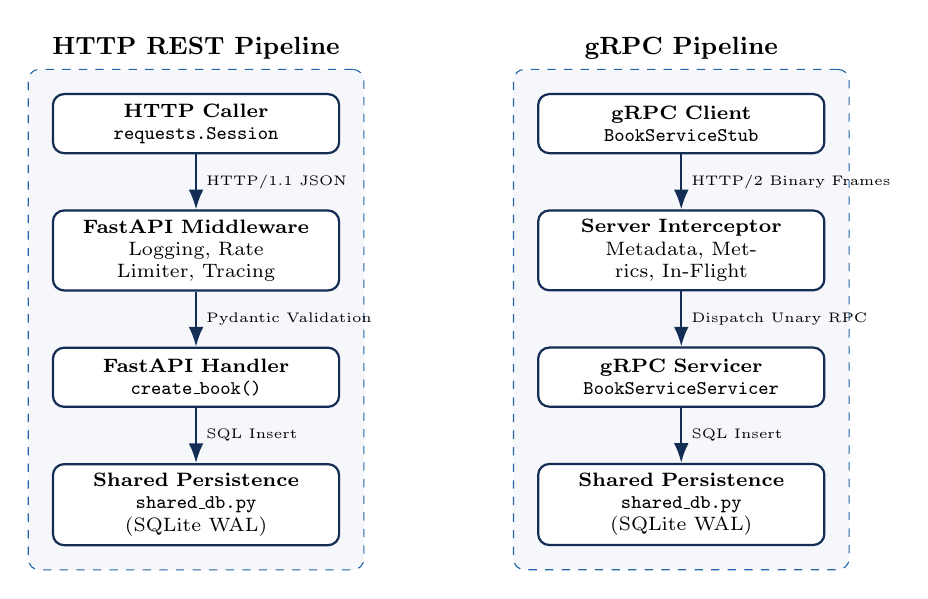
\begin{tikzpicture}[node distance=1.1cm, auto,
    block/.style={rectangle, draw=primary, fill=white, thick, rounded corners, text width=3.4cm, align=center, minimum height=0.75cm, font=\scriptsize},
    layer/.style={rectangle, draw=secondary, fill=lightgray, dashed, inner sep=0.3cm, rounded corners},
    line/.style={draw=primary, -{Latex[length=2.5mm]}, thick}]

    % HTTP Path
    \node [block] (h_client) {\textbf{HTTP Caller}\\\texttt{requests.Session}};
    \node [block, below=0.7cm of h_client] (h_mw) {\textbf{FastAPI Middleware}\\Logging, Rate Limiter, Tracing};
    \node [block, below=0.7cm of h_mw] (h_handler) {\textbf{FastAPI Handler}\\\texttt{create\_book()}};
    \node [block, below=0.7cm of h_handler] (h_db) {\textbf{Shared Persistence}\\\texttt{shared\_db.py} (SQLite WAL)};

    \draw [line] (h_client) -- node [right, font=\tiny] {HTTP/1.1 JSON} (h_mw);
    \draw [line] (h_mw) -- node [right, font=\tiny] {Pydantic Validation} (h_handler);
    \draw [line] (h_handler) -- node [right, font=\tiny] {SQL Insert} (h_db);

    % gRPC Path
    \node [block, right=2.5cm of h_client] (g_client) {\textbf{gRPC Client}\\\texttt{BookServiceStub}};
    \node [block, below=0.7cm of g_client] (g_interceptor) {\textbf{Server Interceptor}\\Metadata, Metrics, In-Flight};
    \node [block, below=0.7cm of g_interceptor] (g_handler) {\textbf{gRPC Servicer}\\\texttt{BookServiceServicer}};
    \node [block, below=0.7cm of g_handler] (g_db) {\textbf{Shared Persistence}\\\texttt{shared\_db.py} (SQLite WAL)};

    \draw [line] (g_client) -- node [right, font=\tiny] {HTTP/2 Binary Frames} (g_interceptor);
    \draw [line] (g_interceptor) -- node [right, font=\tiny] {Dispatch Unary RPC} (g_handler);
    \draw [line] (g_handler) -- node [right, font=\tiny] {SQL Insert} (g_db);

    % Outer groupings
    \begin{scope}[on background layer]
        \node [layer, fit=(h_client) (h_db), label=above:{\small\textbf{HTTP REST Pipeline}}] {};
        \node [layer, fit=(g_client) (g_db), label=above:{\small\textbf{gRPC Pipeline}}] {};
    \end{scope}
\end{tikzpicture}
\caption{End-to-end execution paths comparing HTTP/1.1 REST and gRPC over HTTP/2.}
\label{fig:call_paths}
\end{figure}

\subsection{Semantic Mapping of Status Codes}
Because gRPC operates over HTTP/2 framing, standard HTTP response status lines are replaced by gRPC status codes transmitted in trailing headers. Table~\ref{tab:status_codes} compares the status semantics between both services.

\begin{table}[h!]
\centering
\small
\renewcommand{\arraystretch}{1.25}
\begin{tabularx}{\textwidth}{p{3.2cm} p{2.2cm} p{2.8cm} X}
\toprule
\textbf{Scenario} & \textbf{HTTP Status} & \textbf{gRPC Status} & \textbf{Semantic Mapping Rationale} \\
\midrule
\textbf{Successful Creation} & \texttt{201 Created} & \texttt{OK} (0) & HTTP distinguishes creation (\texttt{201}) from generic reads (\texttt{200}); gRPC uses canonical \texttt{OK} (0) for all successful completions. \\
\textbf{Duplicate Resource} & \texttt{409 Conflict} & \texttt{ALREADY\_EXISTS} (6) & Both indicate conflict against existing database records. Non-transient client fault. \\
\textbf{Invalid Arguments} & \texttt{422 Unprocessable} & \texttt{INVALID\_ARGUMENT} (3) & Indicates malformed payload (e.g., negative price). Both inform the caller not to retry without modifications. \\
\textbf{Resource Missing} & \texttt{404 Not Found} & \texttt{NOT\_FOUND} (5) & 1-to-1 semantic equivalence denoting absent resource identifiers. \\
\textbf{Server Timeout} & \texttt{504 Timeout} & \texttt{DEADLINE\_EXCEEDED} (4) & gRPC propagates explicit deadlines across distributed call chains; HTTP maps timeouts via gateway timeouts. \\
\bottomrule
\end{tabularx}
\caption{Status code mappings between HTTP REST and gRPC services.}
\label{tab:status_codes}
\end{table}

\subsection{Trace Correlation Across Protocol Boundaries}
Structured JSON logging is preserved across both services:
\begin{itemize}\setlength{\itemsep}{0pt}
    \item \textbf{HTTP:} Correlation ID received via \texttt{x-request-id} header (or generated as a UUID) and echoed back in the response header.
    \item \textbf{gRPC:} Extracted from invocation metadata via \texttt{dict(context.invocation\_metadata()).get('x-request-id')}. The server interceptor injects the correlation ID into trailing metadata, outputting uniform JSON logs for Filebeat ingestion:
\end{itemize}
\begin{lstlisting}[basicstyle=\ttfamily\scriptsize]
{"asctime": "2026-10-25 00:15:30", "levelname": "INFO", "name": "bookstore_grpc", "message": "gRPC call processed", "request_id": "grpc-client-d748489e", "service": "bookstore.BookService", "method": "CreateBook", "status": "OK", "duration": 0.0385}
\end{lstlisting}

% =========================================================================
% SECTION 3: PART C
% =========================================================================
\section{Part C: Extending the Metrics}

\subsection{Metrics Audit and Gap Analysis}
Table~\ref{tab:metrics_audit} audits the telemetry pipeline from Assignment 1 and outlines the improvements introduced in Assignment 2.

\begin{table}[h!]
\centering
\small
\renewcommand{\arraystretch}{1.25}
\begin{tabularx}{\textwidth}{p{3.8cm} p{4.8cm} X}
\toprule
\textbf{Metric Name} & \textbf{Assignment 1 State} & \textbf{Assignment 2 Remediation} \\
\midrule
\texttt{books\_created\_total} & Measured total HTTP creations without identifying protocol. & Added bounded label \texttt{protocol} (\texttt{"http"} vs \texttt{"grpc"}), updated atomically by both services. \\
\texttt{books\_in\_inventory} & Gauge tracking catalog size in memory. & Linked directly to shared SQLite WAL storage; updated across both protocols. \\
\texttt{book\_creation\_time\_seconds} & Latency histogram only covering the HTTP endpoint. & Retained for HTTP; created a dedicated \texttt{grpc\_server\_handling\_seconds} histogram with millisecond buckets. \\
\textit{Missing: gRPC Scrape Target} & Zero visibility into RPC traffic or method throughput. & Exposed Prometheus metrics on port \texttt{8001} via \texttt{prometheus\_client.start\_http\_server(8001)}. \\
\textit{Missing: gRPC Status Tracking} & No visibility into RPC errors or failure codes. & Implemented \texttt{grpc\_server\_handled\_total} labeled by \texttt{grpc\_method} and canonical \texttt{grpc\_code}. \\
\textit{Missing: Concurrency Telemetry} & No insight into active connection thread pool load. & Added \texttt{grpc\_server\_in\_flight\_requests} gauge managed by the gRPC interceptor. \\
\textit{Missing: Rate Limiter Telemetry} & Dropped HTTP calls were unrecorded. & Added \texttt{http\_rate\_limited\_total} counter partitioned by endpoint. \\
\bottomrule
\end{tabularx}
\caption{Audit and gap analysis of Assignment 1 metrics.}
\label{tab:metrics_audit}
\end{table}

\subsection{Extended Metrics Specifications}
Table~\ref{tab:metric_specs} specifies all new and revised Prometheus metrics. All metrics strictly adhere to bounded cardinality rules: high-cardinality values such as user IDs, request IDs, and trace IDs are strictly prohibited as Prometheus labels.

\begin{table}[h!]
\centering
\small
\renewcommand{\arraystretch}{1.25}
\begin{tabularx}{\textwidth}{p{3.2cm} p{1.6cm} p{1.2cm} p{2.2cm} p{1.5cm} X}
\toprule
\textbf{Metric Name} & \textbf{Type} & \textbf{Unit} & \textbf{Bounded Labels} & \textbf{Origin} & \textbf{PromQL Query} \\
\midrule
\texttt{grpc\_server\_handled\_total} & Counter & calls & \texttt{grpc\_method}, \texttt{grpc\_code} & Server & \texttt{sum(rate(grpc\_server\_handled\_total[1m])) by (grpc\_method, grpc\_code)} \\
\texttt{grpc\_server\_handling\_seconds} & Histogram & seconds & \texttt{grpc\_method}, \texttt{le} & Server & \texttt{histogram\_quantile(0.95, sum(rate(grpc\_server\_handling\_seconds\_bucket[5m])) by (grpc\_method, le))} \\
\texttt{grpc\_server\_in\_flight\_requests} & Gauge & calls & \texttt{grpc\_method} & Server & \texttt{grpc\_server\_in\_flight\_requests} \\
\texttt{http\_rate\_limited\_total} & Counter & reqs & \texttt{endpoint} & Server & \texttt{rate(http\_rate\_limited\_total[1m])} \\
\texttt{books\_created\_total} & Counter & items & \texttt{protocol} & Server & \texttt{sum(rate(books\_created\_total[1m])) by (protocol)} \\
\bottomrule
\end{tabularx}
\caption{Prometheus metrics specifications for Assignment 2.}
\label{tab:metric_specs}
\end{table}

\noindent\textbf{Design Choice: In-Flight Requests vs. Message Size:}\\
We chose \textbf{In-Flight Requests (\texttt{grpc\_server\_in\_flight\_requests})} over Message Size because gRPC utilizes multiplexed HTTP/2 streams over persistent TCP connections. In production, head-of-line blocking and thread-pool exhaustion occur when concurrent calls back up against slow database locks. Tracking in-flight requests provides an immediate leading indicator of saturation before CPU thresholds are crossed. Because bookstore catalog messages have small, predictable payload sizes (200--500 bytes), message size metrics offer minimal diagnostic value by comparison.

\subsection{Prometheus Scrape Configuration and Grafana Telemetry}
The updated Prometheus configuration (\texttt{prometheus.yml}) scrapes both services concurrently:
\begin{lstlisting}[basicstyle=\ttfamily\scriptsize]
scrape_configs:
  - job_name: 'bookstore-api'
    static_configs:
      - targets: ['api:8000']
  - job_name: 'bookstore-grpc'
    static_configs:
      - targets: ['grpc-service:8001']
  - job_name: 'node-exporter'
    static_configs:
      - targets: ['node-exporter:9100']
\end{lstlisting}

\noindent Figures~\ref{fig:grafana_1},~\ref{fig:grafana_2}, and~\ref{fig:grafana_3} present the live Grafana dashboard populated using the repeatable traffic burst generator (\texttt{traffic\_generator.py --mode metrics}).

\begin{figure}[h!]
    \centering
    \includegraphics[width=0.92\textwidth]{figures/grafana_overview_1.png}
    \caption{Grafana Dashboard: Book Creation Rate, Inventory Gauge, and gRPC Method Throughput side-by-side.}
    \label{fig:grafana_1}
\end{figure}

\begin{figure}[h!]
    \centering
    \includegraphics[width=0.92\textwidth]{figures/grafana_overview_2.png}
    \caption{Grafana Dashboard: Response latencies (p95 HTTP vs. gRPC p50/p95 histograms) and in-flight active concurrency.}
    \label{fig:grafana_2}
\end{figure}

\begin{figure}[h!]
    \centering
    \includegraphics[width=0.92\textwidth]{figures/grafana_overview_3.png}
    \caption{Grafana Dashboard: HTTP Rate-Limiting rejections (429s) plotted alongside cross-protocol creation volume.}
    \label{fig:grafana_3}
\end{figure}

% =========================================================================
% SECTION 4: CONCLUSION
% =========================================================================
\section{Conclusion}
Assignment 2 successfully transitioned the Bookstore service from a basic monolithic prototype into an enterprise-grade, dual-protocol platform. We validated REST architectural constraints, eliminated duplicate-submission hazards through idempotency caching, protected service capacity using sliding-window rate limiting, and demonstrated client resilience with exponential backoff and a three-state circuit breaker. The introduction of a dedicated gRPC microservice backed by SQLite WAL persistence proved that binary HTTP/2 framing can coexist with HTTP/1.1 REST without data fragmentation. Finally, extending the Prometheus and Grafana telemetry pipeline with method-level status codes, latency histograms, and concurrency gauges establishes end-to-end observability across the entire system.

\end{document}
